\subsection{Normalmapping}
\label{section:Normalmapping}

Um die visuelle Qualität eines Models zu erhöhen, so muss man das Modell genauer modellieren und somit resultieren mehr Dreiecke. 
Damit erhöht sich aber auch der Rechenaufwand für dieses Model und ab einer bestimmten Grenze ist die gewonnene Qualität nur sehr gering, der Rechenaufwand aber um so größer. Um ein Model trotzdem noch hochauflösender darzustellen wird ein Vorgang namens \textit{Normalmapping} verwendet. 
Dieser baut auf Lichtberechnungen auf, denn ohne Licht gibt es keine zu erkennende verbesserte Qualität. Normalerweise hat jeder Vertex einen Normalenvektor und für einen Pixel wird er zwischen den 3 Vertices interpoliert. Mit Normalmapping weißt man jedem Pixel einen eigenen Normalenvektor zu, so ist es möglich die Oberfläche so aussehen zu lassen, als würde sie rau mit kleinen Unebenheiten sein, ohne den Rechenaufwand von dem Rendern vieler Dreiecke eines Meshes zu belasten.
Den Unterschied Sieht man in \cref{img:Normalmapping}. Die Normalenvektoren werden in einer Textur gespeichert, sodass sie mit den normalen Texturen-Koordinaten verwendet werden können. Diese Textur wird im Material abgespeichert.

In einer Textur können drei Werte abgespeichert werden, Rot, Grün und Blau, jeweils mit einem Wert von 0 bis 1. Ein Normalenvektor hat aber drei Komponenten mit jeweils Werten von -1 bis 1, daher muss dieser erst berechnet werden:

$ \overrightarrow{N} = 
\begin{pmatrix}
x \\ y \\ z
\end{pmatrix}
 = 2 \cdot \overrightarrow{C} - 1 = 
 \begin{pmatrix}
 2 \cdot r - 1 \\ 2 \cdot g - 1 \\ 2 \cdot b - 1
 \end{pmatrix}$
 
Der Normalenvektor $\begin{pmatrix}
	0 \\ 0 \\ 1
\end{pmatrix}$ zeigt direkt weg von dem Model, daher sind Normalmaps auch immer sehr bläulich, denn der meiste Anteil des Normalenvektors liegt in der Z-Komponente. Eine Beispiel Normalmap ist in \cref{img:Normalmap} zu sehen. Man kann diesen Vektor aber nicht direkt verwenden, da er im \textit{Tangent space} definiert ist. Dies bedeutet dass er relativ zu dem zugehörigen Dreieck steht.
Man benötigt zudem einen Normalenvektor im \textit{Object space}, also relativ zu dem Model. 
Zur Umwandlung wird eine 3x3 Matrix benötigt, die aus drei verschiedenen Vektoren des Tangent-Space gebildet wird. 
Es können hierbei drei beliebige nicht linear abhängige Vektoren verwendet werden. Man bemerkt schnell, dass wenn alle drei orthogonal zueinander verlaufen, es simpler und effizienter ist die Matrix zu erstellen. 
Der erste Vektor wird bereits angegeben. Dieser beschreibt den Standardnormalenvektor jedes Vertex. Hinzu kommt noch ein Tangentenvektor jedes Vertex. Dieser befindet sich ebenfalls im \ac{VBO} des Meshes, wie in \cref{table:VertexAufbau} abgebildet ist. Der dritte Vektor ist der Bitangentenvektor
und kann mittels Kreuzprodukt aus diesen beiden berechnet werden. Es ist nötig alle drei Vektoren zu normalisieren, bevor die Matrix erstellt wird.

Gegeben ist der Normalenvektor $\overrightarrow{N}$ und der Tangentenvektor $\overrightarrow{T}$

Die normalisierten Vektoren: $\overrightarrow{N_{0}} = \dfrac{\overrightarrow{N}}{|\overrightarrow{N}|}$\qquad	$\overrightarrow{T_{0}} = \dfrac{\overrightarrow{T}}{|\overrightarrow{T}|}$

Der Bitangentenvektor: $\overrightarrow{B} = \overrightarrow{N_{0}} \times \overrightarrow{T_{0}}$\qquad	$\overrightarrow{B_{0}} = \dfrac{\overrightarrow{B}}{|\overrightarrow{B}|}$

Die Matrix sieht dann so aus: $M =  \begin{pmatrix}
T_{0x} & B_{0x} & N_{0x} \\
T_{0y} & B_{0y} & N_{0y} \\
T_{0z} & B_{0z} & N_{0z} \\
\end{pmatrix}$

Diese Matrix wird für erhöhte Leistung im Vertex shader erstellt und dann dem Fragment shader übergeben. In diesem muss dann nur der Normalenvektor aus der Normalmap geladen werden, dafür werden die gleichen Texturekoordinaten verwendet wie bei der Color texture, und mit dieser Matrix multipliziert werden.

\begin{figure}
	\begin{center}
		\includegraphics[width=0.5\textwidth]{02theorie/Normalmapping.png}
		
		Oben: mit Normalmapping, Unten: ohne Normalmapping
		
		Model: Allosaurus aus dem Spiel "`Ark: Survival Evolved"
		
		\caption{Normalmapping Beispiel}
		\label{img:Normalmapping}
	\end{center}
\end{figure}
\begin{figure}
	\begin{center}
		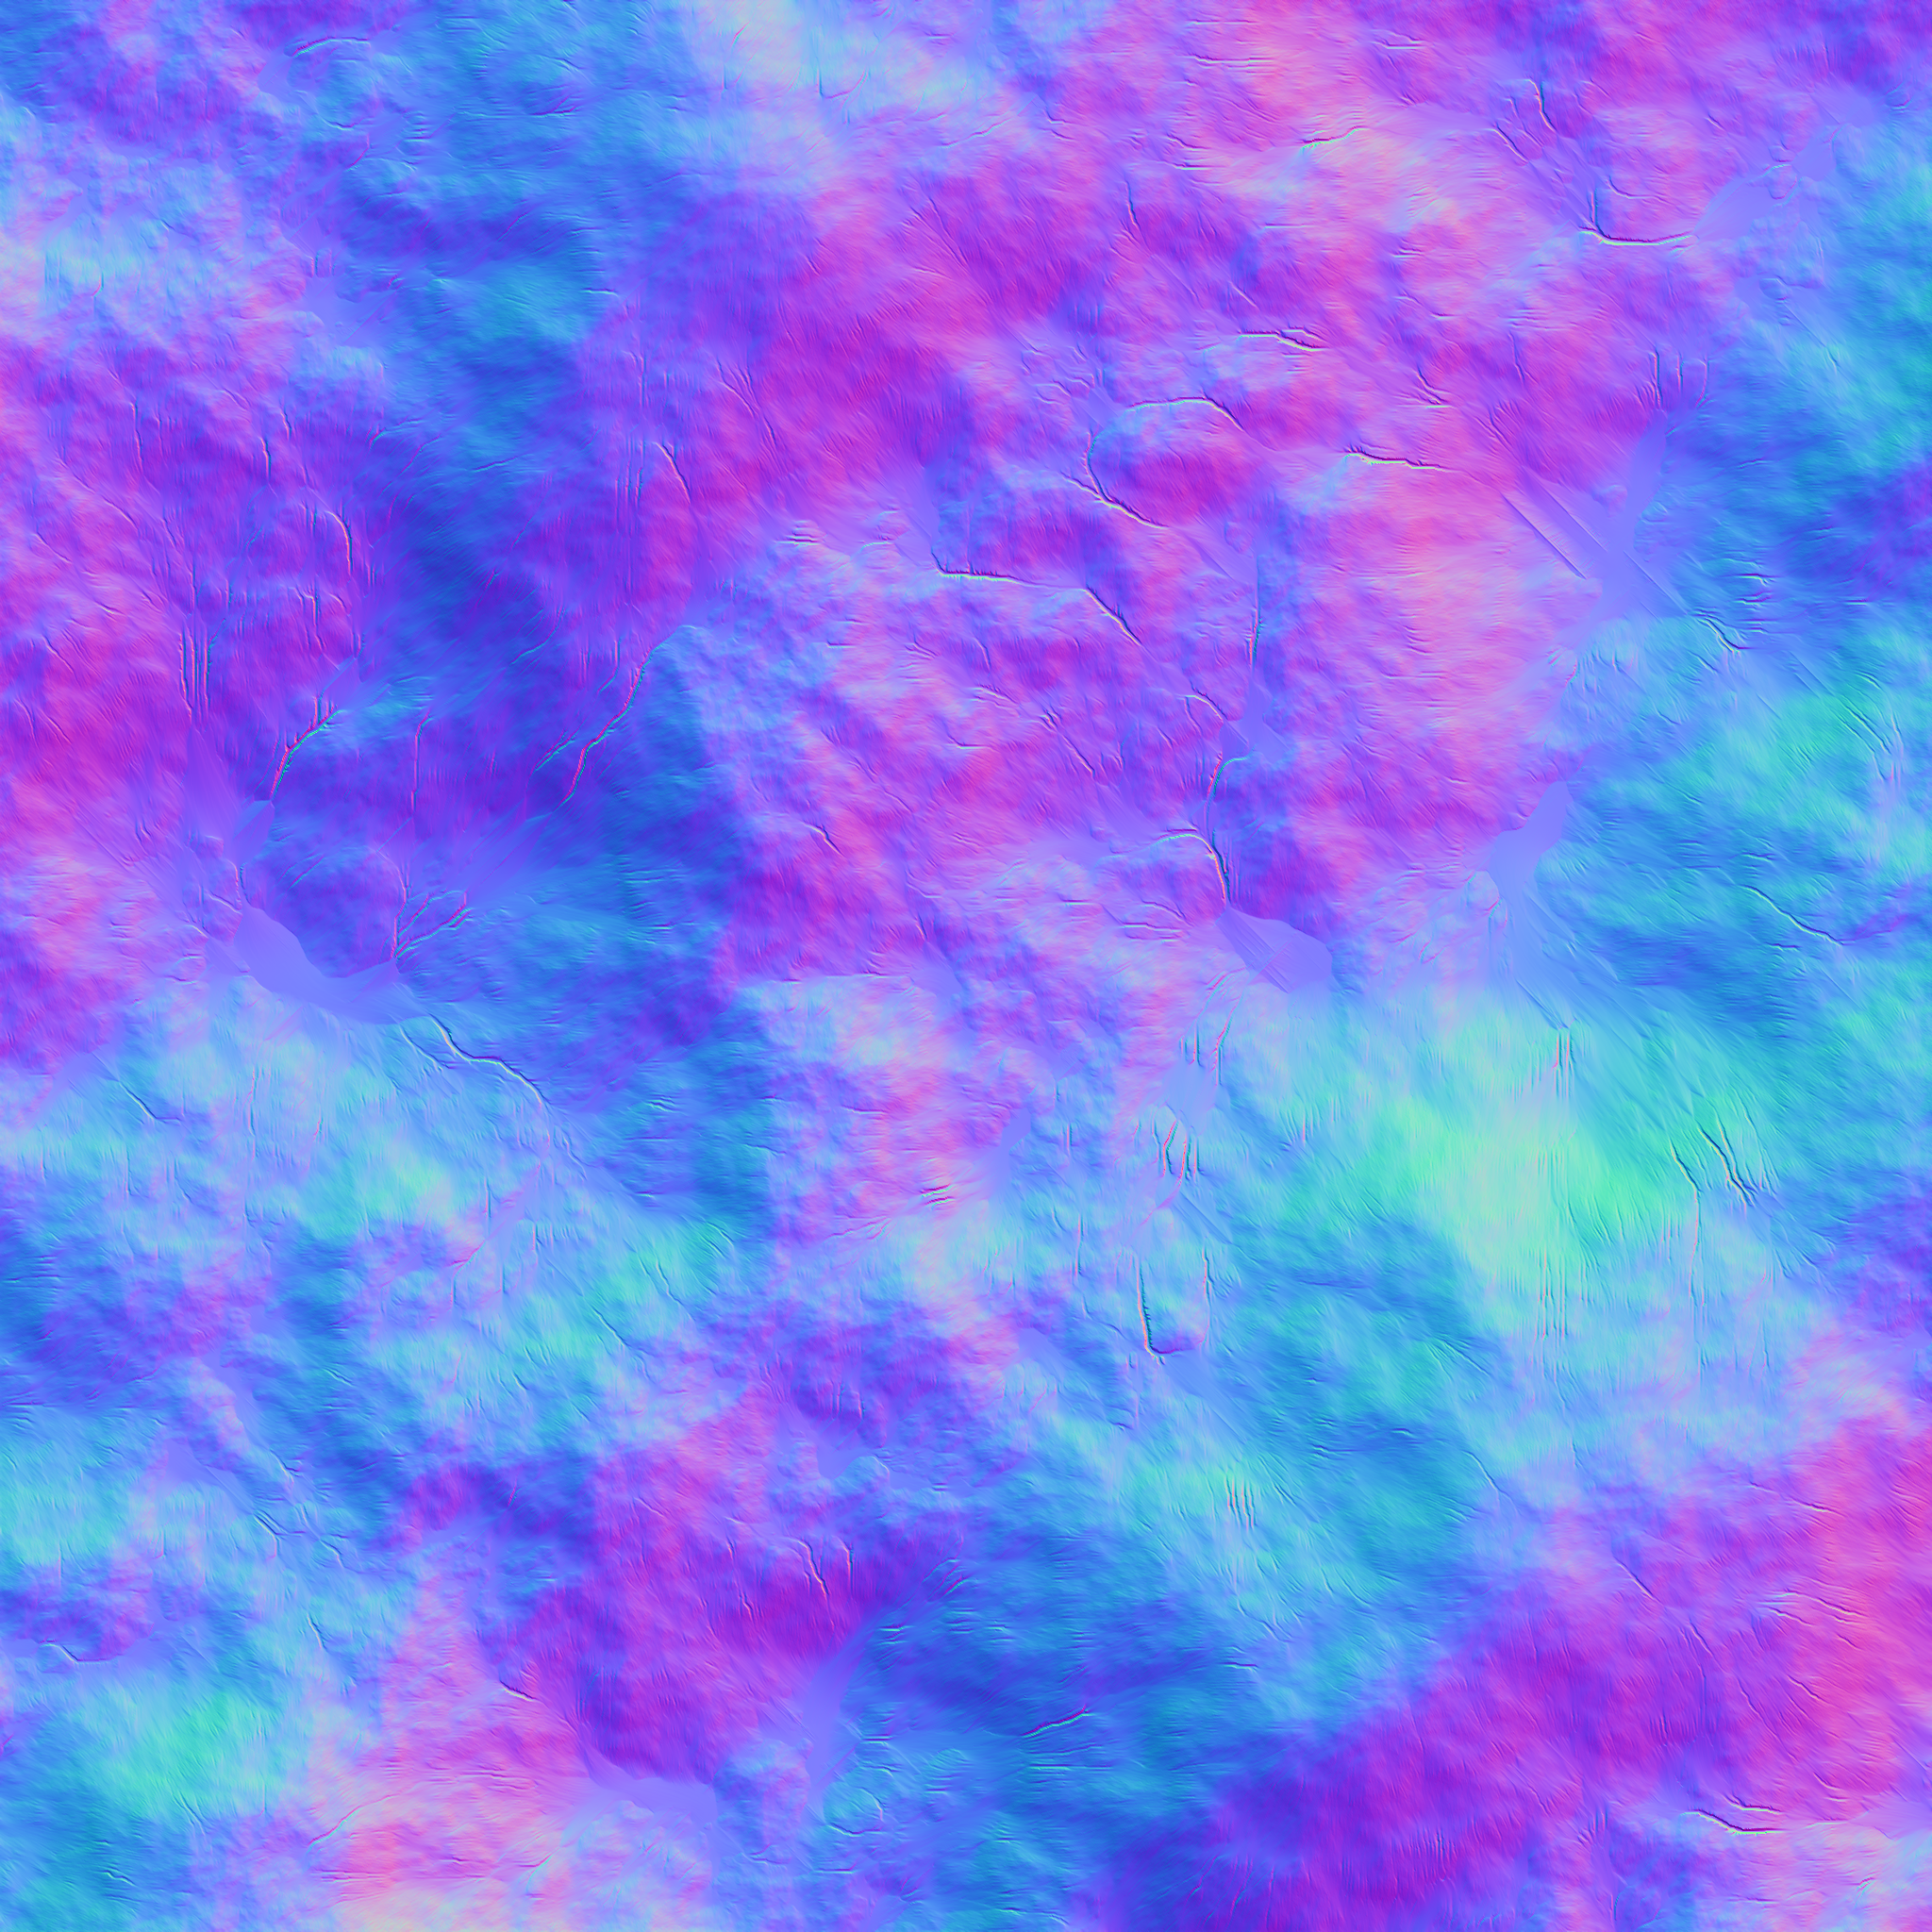
\includegraphics[width=0.4\textwidth]{02theorie/normalmap.png}
		
		Eine Beispiel Normalmap
		
		Quelle: http://www.bencloward.com/images/tutorial\textunderscore normals07.gif
		
		\caption{Normalmap Beispiel}
		\label{img:Normalmap}
	\end{center}
\end{figure}